\section{Development}
	In this section I will cover development of the product as well as the software engineering methods and tactics used.
	
	\subsection{Methods}
		In this section I will specify methods used in the development period for this project.
		\subsubsection{Time \& Cost}
			Accurate time and cost estimation is a persistent challenge in software development. Common methods include:
			\begin{itemize}
				\item Expert methods, such as Delphi Technique, Planning Poker, Analogous Estimating, and Expert Judgement.
				\item Algorithmic Methods, such as COCOMO, Function Point Analysis, and Use Case Points.
			\end{itemize}
			Each method has strengths depending on project scope, team size, and experience. For this project, Expert Judgment is used, as the technologies involved are familiar. This allows for reliable estimates of feature development time.
			
			For larger or less technology specific experienced teams, a different method may be more suitable, as Expert Judgment relies heavily on prior experience.\\
		
			To select the next feature for implementation, dependencies between planned features are evaluated, along with the user value each feature provides. A cost-benefit assessment is conducted at the start of each iteration to ensure the project remains aligned with its scope.
		
		\subsubsection{Development model}
			Software development is often guided by two main methodologies: Waterfall and Agile. Waterfall is suitable when requirements are unlikely to change, such as in medical software. Waterfall is a method for when requirements is not likely to change such as developing medical software. Waterfall often follows these steps:
			\begin{figure}[!h]
				\begin{center}
					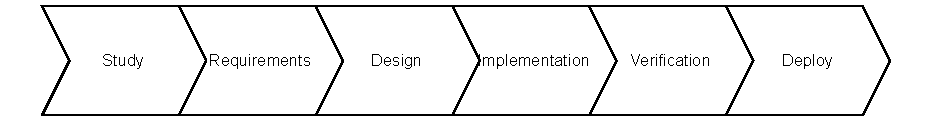
\includegraphics[width=.8\textwidth]{Images/Waterfall}
					\caption{Waterfall Workflow}
					\label{fig:waterfall}
				\end{center}
			\end{figure}
	
			Agile is more adaptive and supports frequent changes in requirements. The stages in agile is often circular and allows for going back and forth in the stages.
			
			This project applies some SCRUM practices, with iterations limited to two weeks. After each iteration, the project state is reviewed to support requirement adjustments. The first day of each iteration is reserved for documentation and reflection on the previous cycle. The class diagram is updated regularly to maintain a clear overview of the system.
			
			Maintaining a high-level overview enables early identification of flawed implementations, allowing timely corrections before issues escalate.\\
	
			\begin{figure}
				\begin{center}
					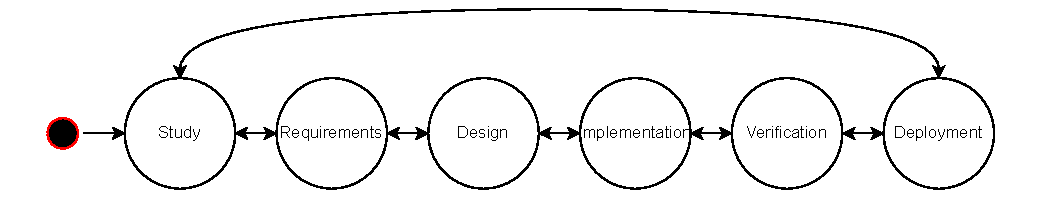
\includegraphics[width=\textwidth]{Images/Iterative}
					\caption{Iterative Workflow}
					\label{fig:iterative}
				\end{center}
			\end{figure}
	
	\subsection{Process}
		\textbf{Tools}\\ \noindent
			Tools that monitor memory and CPU usage can help identify problems or bottlenecks early in the development process. Additional tools are developed and used to accelerate testing and experimentation. A custom \gls{gui} was created to streamline testing by enabling easy deployment of a varied set of test cases. Docker is used for experiment deployment, as it also provides the ability to track CPU, memory, and network usage.\newline \newline
		\noindent

	\subsection{Analysis}\label{sec:Analysis}
		To determine the optimal design based on insights from the research phase, several analytical methods are applied.
		First, features are separated into those likely to provide value to the end user and those considered less relevant. This is done through brainstorming, as other methods are less effective in producing satisfactory results according to the developers experience.
	\subsubsection{Potiential Features}
	\begin{itemize}
		\item Modability during run-time : The idea here being that a user would never need to have any downtime even when they only run one instance of \gls{reps}. This would lean towards a component based design of \gls{reps}, but could be implemented through other means.
		\item Adding or removing nodes during run-time : This comes with the same general idea which could reduce down time when using only one instance.
		\item Hybridize with other predictive models : Someone could insert a \gls{ml} model while still keeping memory usage low, this would allow \gls{reps} to extremely complex in is design and cover a large use case. It can be imagined that \gls{reps} already is going to require a large usage of memory, therefore models which is memory demanding such as \gls{knn} will be unusable in a \gls{reps}.
	\end{itemize}
	
	\subsubsection{Requirements}\label{sec:Requirements}
	Here I will determine the requirements through a MoSCoW analysis. The goal of this analysis is to determine the priority of features and it will lead to what technology that I will be using throughout this project. As I will base the technology choice on their ability to satisfy these requirements.\\
	A clear project scope is defined early to maximize the value of collected experience and data from this project. Therefore a MoSCoW analysis is used to prioritize features.\\
	Functional Requirements:
	\begin{center}
		\resizebox{.9\textwidth}{!}{
			\scriptsize
			\begin{tabular}{|p{2cm}|p{3cm}|p{2cm}|p{3cm}|p{3cm}|p{2cm}|}
				\hline
				Requirement ID & Requirement & Prioritization Level & Description & Reason & Comments \\ \hline
				FR0 & Having individual process in each 'Event Node' & Must have & An 'Event Node' is the main process of make predictions and conclusions & It is the point that these process' can be used to make predictions and conclusions & \\ \hline
				FR1 & Is able to communicate with others services which is not part of the REPS & Must have & Other system must be able to get values from REPS to make determinations based on the states REPS notices & For other system can react based on the states REPS notices, it need to share it, otherwise there is no need for REPS & \\ \hline
				FR2 & Being able to easily add new 'Event Nodes' & Could have & Using XML, JSON or a third option, one could easily add new nodes to the REPS System & It could speed up testing, but it is not a requirement for the system to function & This would require FR3 \\ \hline
				FR3 & Being able to quickly spin up \gls{reps} using a specific file type & Could have & Could allow for implementing the system quicker and allow for sharing REPS' &  It could speed up testing, but it is not a requirement for the system to function & \\ \hline
				FR4 & Allow for ML Models in the 'Event Nodes' & Should have & This could really expand the use cases for \gls{reps} as companies may have their own or develop one for their problem & It is very useful for this project, but not required to be seen as successful & \\ \hline
				FR5 & Able to detect events & Must have & Detect any events occurring in the system & This is the whole point of the system & \\ \hline
				FR6 & Graphical user-interface & Wont have & A user interface can make it easy for the developer to setup REPS & This would require too much time without giving anything useful to determine the viability of the system & \\ \hline
				FR7 & Automatic \gls{reps} creation & Wont have & It could in theory make it so a system could automatically create a REPS based on system documentation & This is a research topic in itself and is too add this to the project & \\ \hline
			\end{tabular}
		}
	\end{center}
	{\scriptsize Wont have means I do not plan to implement such feature at the moment, but is included as this could have value for future work.}
	
	\begin{center}
		\resizebox{.9\textwidth}{!}{
			\scriptsize
			\begin{tabular}{|p{2cm}|p{3cm}|p{2cm}|p{3cm}|p{3cm}|p{2cm}|}
				\hline
				Requirement ID & Requirement & Prioritization Level & Description & Reason & Comments \\ \hline
				NF0 & Should not have a high complexity & Should have & high complexity is in terms of the developer being able to understand the system & The advantage with this is the developer should be able to understand how a decision is made compared to most MLs. & \\ \hline
				NF1 & Restricted Memory usage & Could have & Risk of high resource usage & I fear that this system might suffer from memory in smaller computers & \\ \hline
				NF2 & Easy to communicate with & Should have & Should be easy to gain the values which is needed from the REPS & It would make it hard on the people using REPS if this requirement is not fulfilled, diminishing the use fullness of REPS & \\ \hline
			\end{tabular}
		}
	\end{center}
	
	\subsubsection{Technology Choices}\label{sec:TechChoices}
	Based on these requirements, it is deemed that that the following technologies, frameworks and patterns is needed:
	\begin{itemize}
		\item Publish Subscribe pattern, MQTT (FR1, FR2, FR3, NF2):\\
		A publish subscribe pattern fits best when it comes to communication, the modifiability and adaptability that comes with this pattern fits very well with the communication requirement (FR1) while also allowing for easy adaptability (FR2 \& FR3). I want a light weight solution, I there don't see a need for kafka.
		\item JSON interpreter for saving (FR2, FR3):\\
		A relational database doesn't fit with the way REPS is built. The adaptability with JSON or XML will work great with REPS. There neither a need for the performance from a relational database. I will be using JSON as I have implemented similar features in JSON several times, while I've done i far less in XML. I will neither be using AVRO due to the increased time cost.
		\item C\#:\\
		I have most experience with this, it may be slower than other compiled languages such as C/C++, but it is fast enough to achieve the goals for this project. I also believe that it being object oriented language fits well with REPS. Only drawback I see is that not a lot of ML are developed for C\# compared to python. This will limit the time of implementing FR4, but will allow me to quicker implement all other features.
		\item Roslyn:\\
		TODO
		\item \gls{ml} models:\\
		TODO
	\end{itemize}
	\newpage
	\begin{figure}[!h]
		\begin{center}
			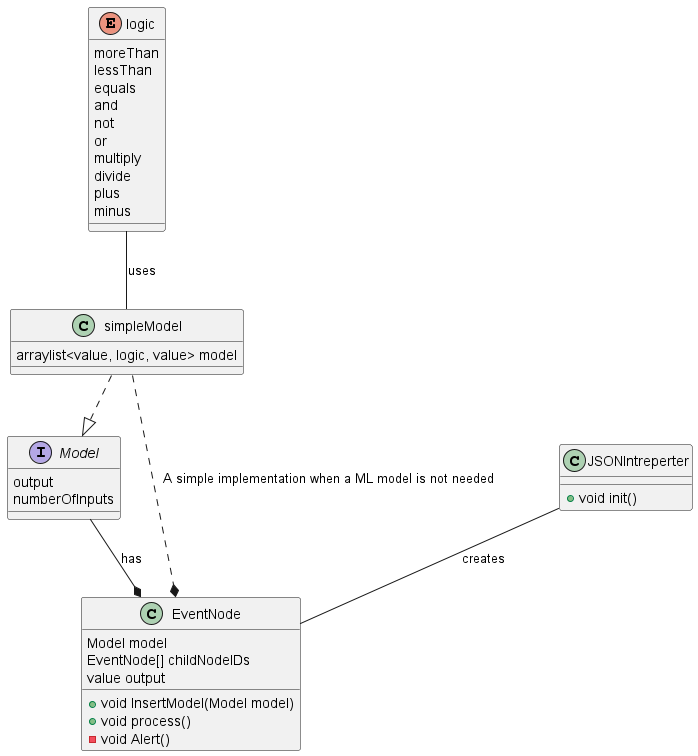
\includegraphics[width=.5\textwidth]{Images/AnalysisClassDiagram}
			\caption{First Iteration Design Diagram}
			\label{fig:analysisDiagram}
		\end{center}
	\end{figure}
	
	Based on the diagrams from Figure \ref{fig:analysisDiagram}, I will be using RabbitMQ for MQTT due to it supporting all needs for this project while being able to be implemented in C\#. It supports all classic MQTT features, but also it support Queue priority which I believe will be necessary in a crisis situation. There should be a limit to the amount of priority levels, as the higher the max is set, the more CPU resources is required. Also some messages which should expire might be stuck as rabbitMQ expires from the head of the queue. Now I don't believe this will be a problem as long as the end user doesn't send too many messages.
	
	For C\# I will have to use the 'Object' type for the output, I could be using the 'dynamic' type, but as it is casted in runtime to the type that I would might need. I cannot define it as a 'var' type because that would still be defined during compile time, and it has to be defined during runtime. Now using object I will have to define a set og legal casting types, so I will lose flexibility but I severely decrease the risk of runtime errors with this variable.
	
	I will be using C\#'s Roslyn to interpret a function during runtime. This will allow for full customisation in terms of math and if statements.
	
	The await function releases current thread and allows for the REPS model to operate as a tree when it comes to their dependencies, as a Event node requires that the former events has processed before processing itself.
	
	For \gls{json} reading, I'll be using Newtonsoft which is a C\# framework for interpreting JSON. The choice for this is due to its easiness, vast documentation, and is the most downloaded nuget package [https://www.nuget.org/PACKAGES?q=\&includeComputedFrameworks=true\&prerel=true\&sortby=totalDownloads-desc], which means that if a problem were to occur, that a solution to that problem would most likely exist on stackoverflow or similar sites.
	
	(TODO: gennemgå flere af noterne og skriv om rabbitMQ og threading begrundelserne her)
	
	\subsection{Design}
	Based on the analysis (\ref{sec:Analysis}), a set of technology choices (\ref{sec:TechChoices}) could be stated which is needed to achieve the requirements (\ref{sec:Requirements}). Based on the technology, a more precise design is made to align with the technology.
	\begin{figure}[!h]
		\begin{center}
			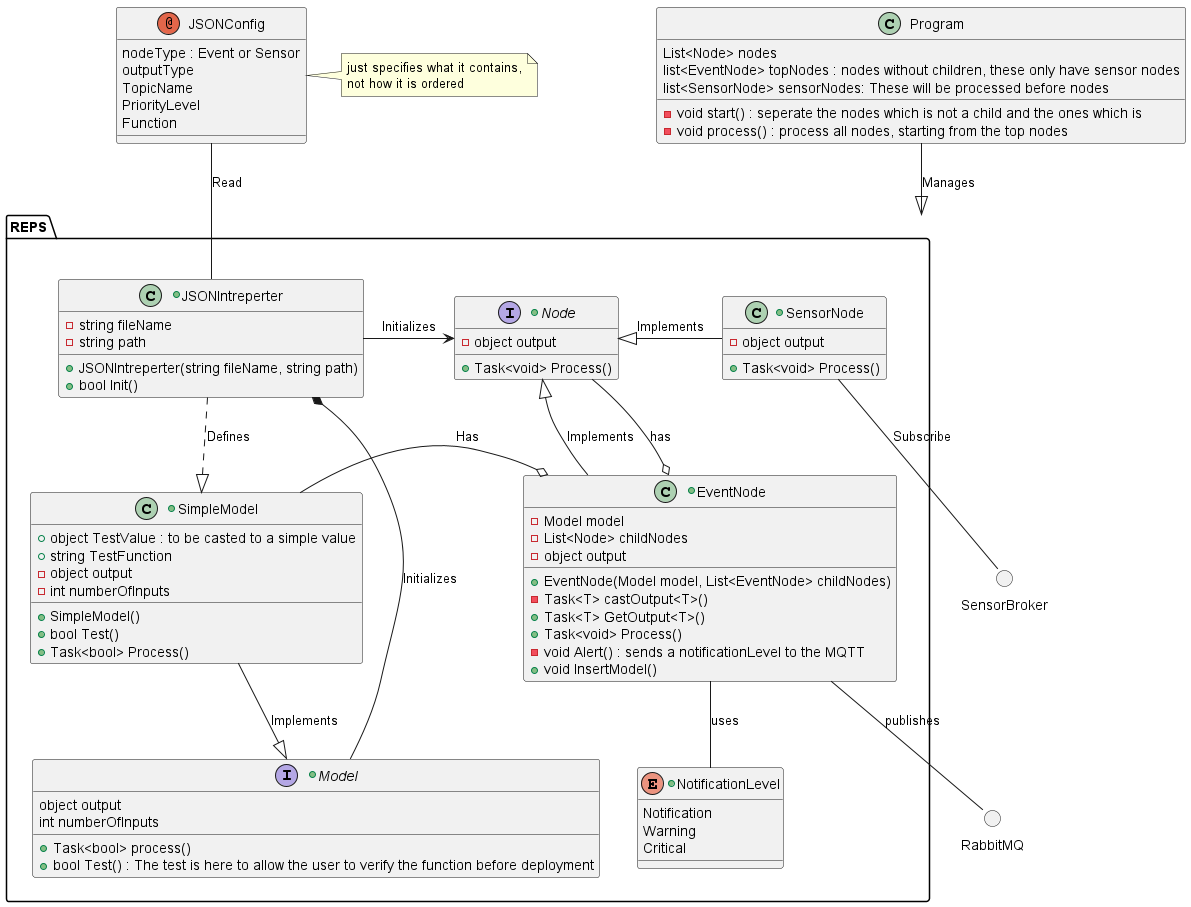
\includegraphics[width=.9\textwidth]{Images/DesignAnalysisDiagram}
		\end{center}
	\end{figure}
	
	\begin{figure}[!h]
		\begin{center}
			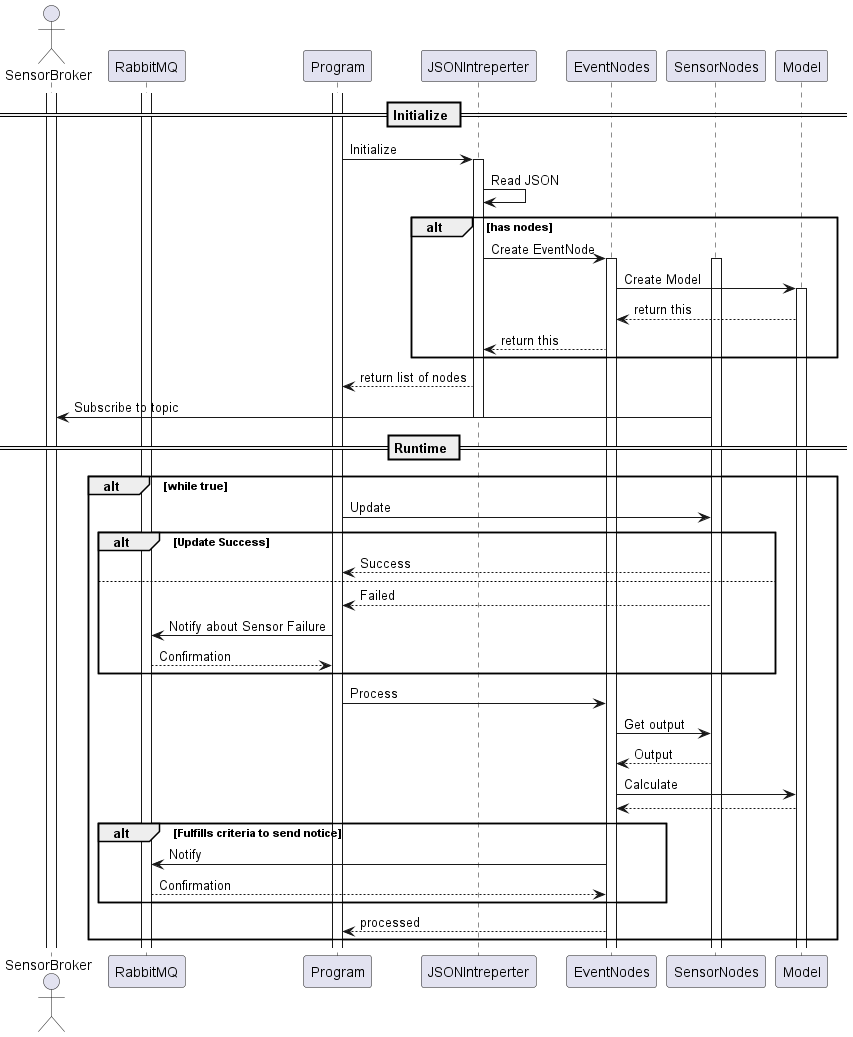
\includegraphics[width=.6\textwidth]{Images/SequenceDiagram}
			\caption{Sequence Diagram}
		\end{center}
	\end{figure}
	
	As the project furthers and new iterations of the project is completed, the class diagram will be updated with the final diagram:
	
	\begin{figure}[!h]
		\begin{center}
			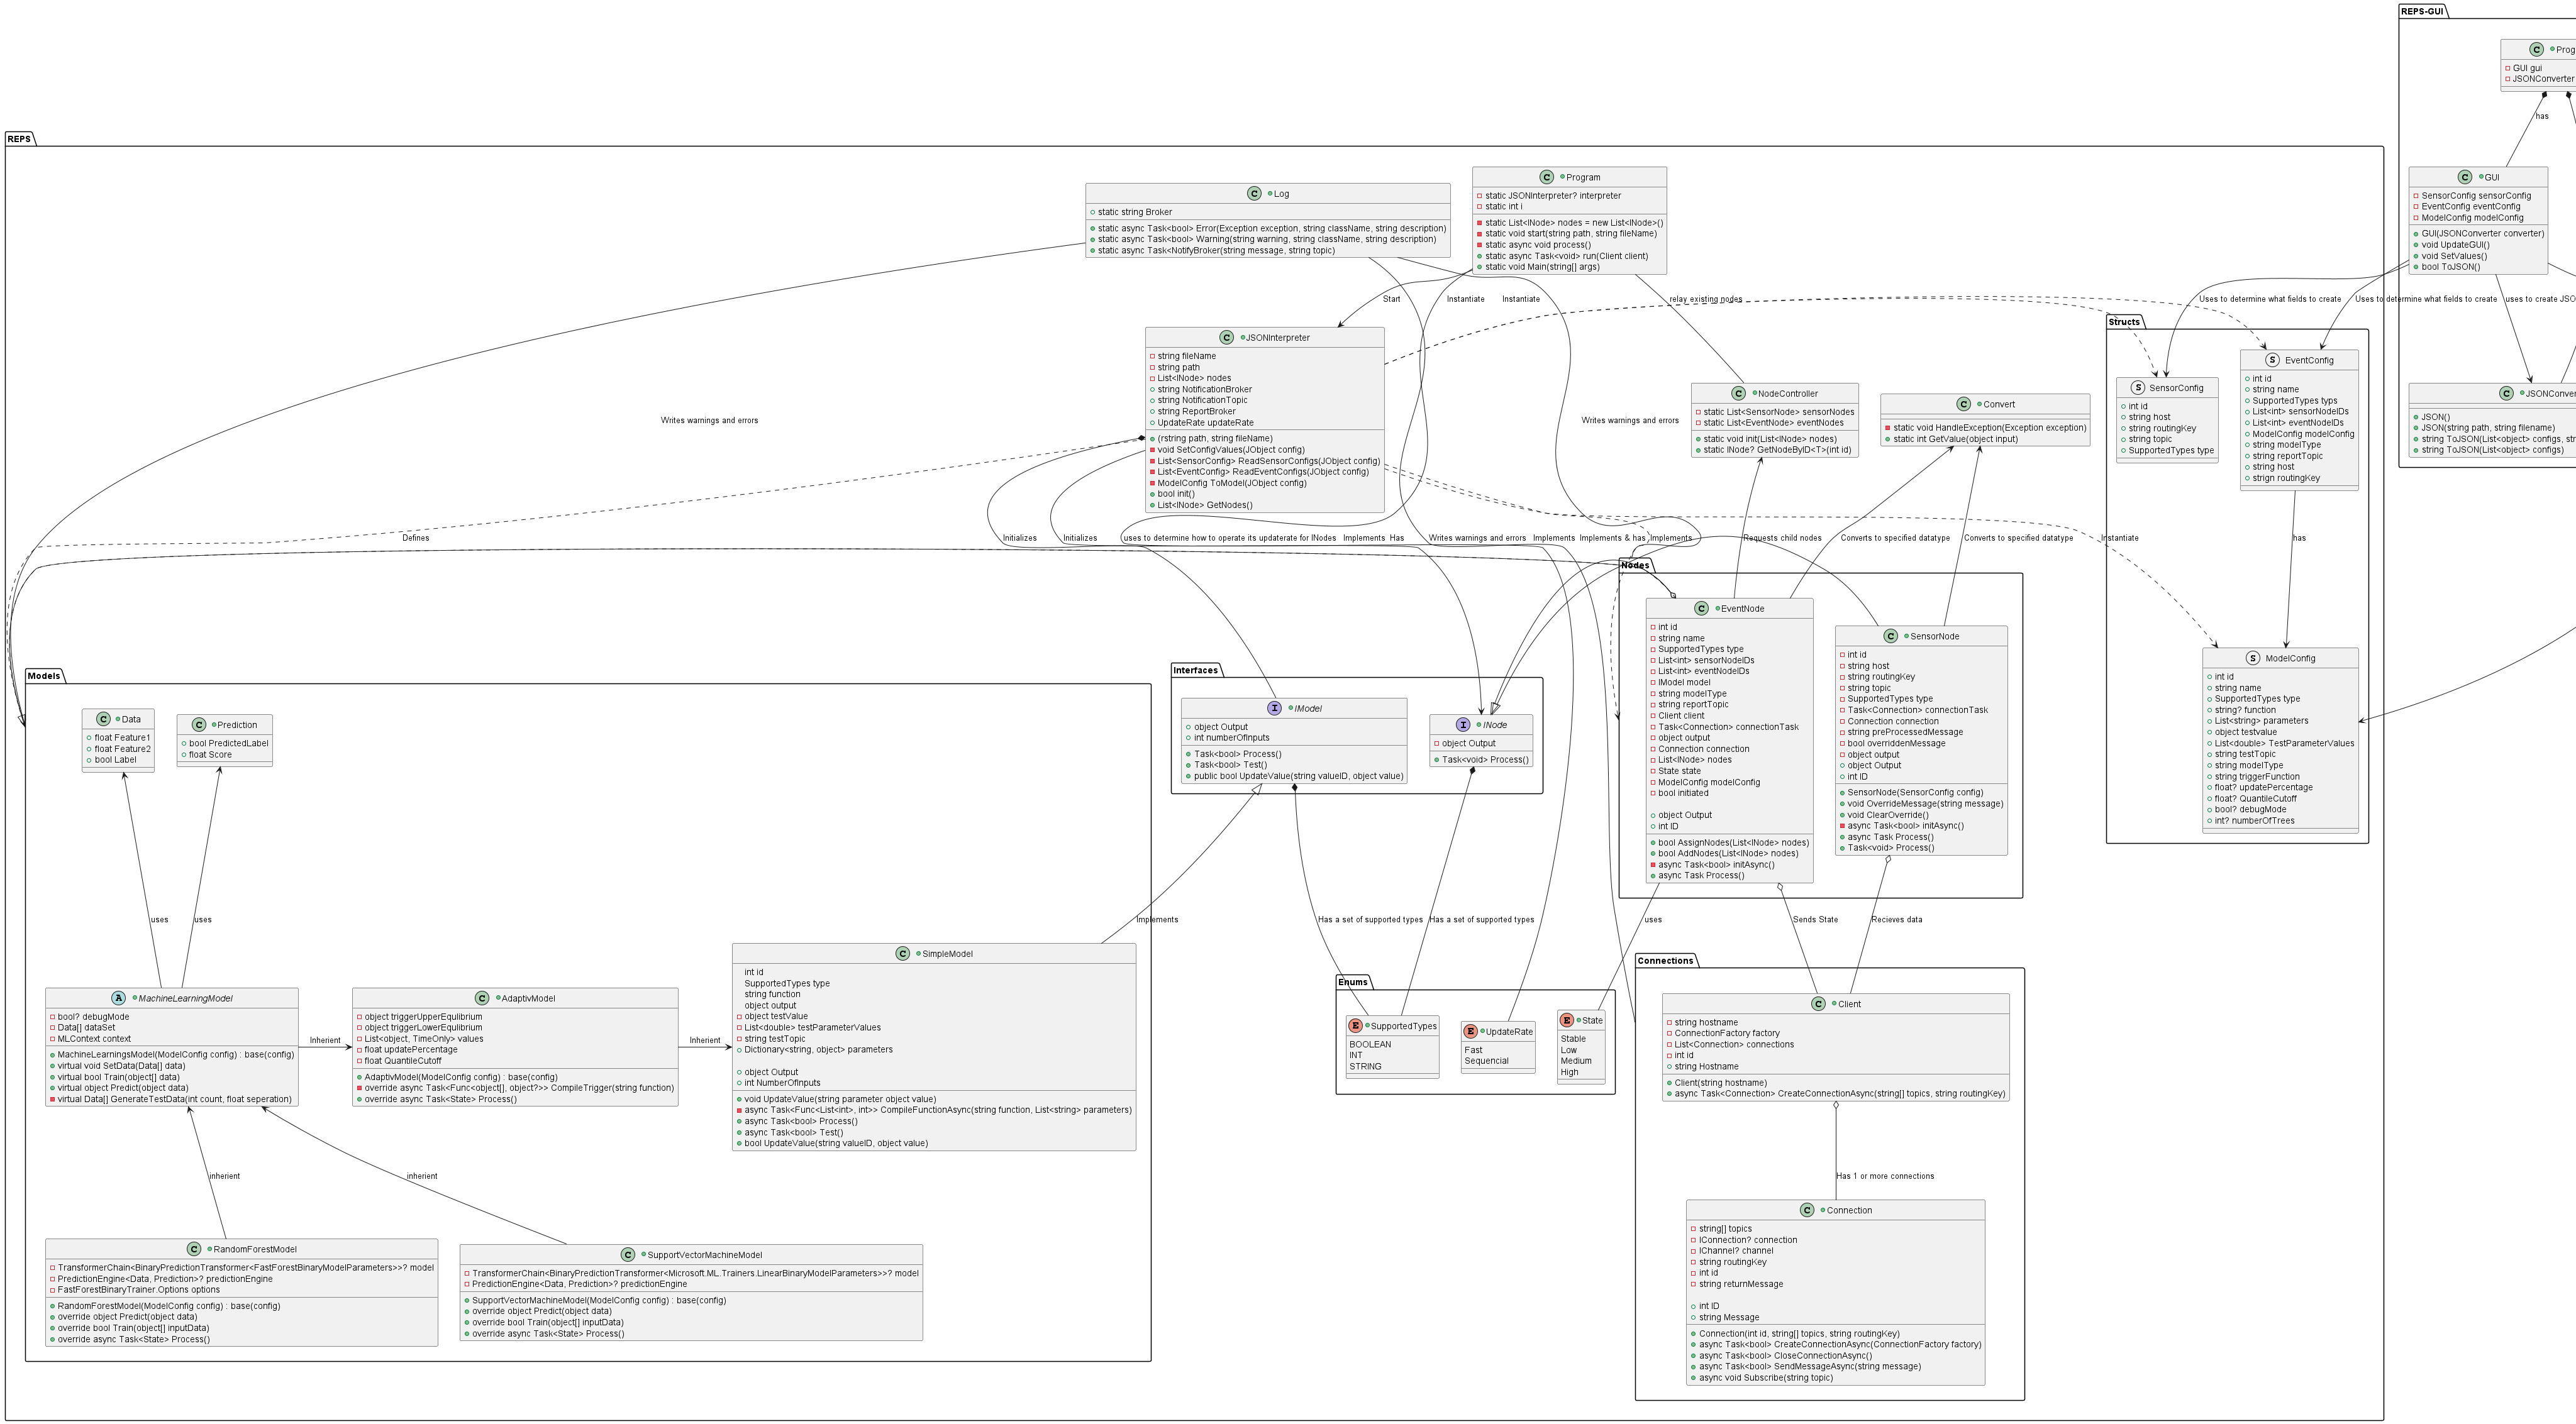
\includegraphics[width=.8\textwidth]{Images/Latest}
			\caption{Final ClassDiagram}
			\label{fig:FinalClassDiagram}
		\end{center}
	\end{figure}
	UPDATE Latest image!\\
	(TODO: Fix image layouttet)

	The \gls{reps} is split up in 2 parts, the system itself and then a \gls{gui}.\newpage 
	
	
		\noindent
		\textbf{Logical Insurance}\\
		To ensure the correctness of the system's logic, UPPAAL, a model-checking tool is used to validate the system's logic before implementation. This reduces the risk of introducing logical errors early in development.\\
	\subsection{REPS Implementation}\label{Reps:Imp}
	\gls{reps} starts with loading a config file, this file is in the form of JSON. JSON was used due to how easy it is to modify between tests as well as it being a type which can function with other systems such as the \gls{gui}. It will create the different nodes from this JSON config, these configs are structs containing all of the data for their respective nodes. A sensor node receives data from a sensor or through another communication method. It was determined that the nodes should make use of publish subscribe pattern as this fits with the dynamic nature of the nodes. I used RabbitMQ for all communication due to it supporting priority queuing. An Event node retrieves the data from the sensor nodes to then use in their model, the output of this model is then made available to other nodes. A Event node also has a Trigger function which is used to determine severity of the ongoing event.
	
	Each Node will make a connection to the MQTT broker with a specific topic which it either publishes to or retrieves data from. An Event node publishes to the broker depending on the severity of the event and user preferences.
	
	\subsubsection{Models}
	Models uses C\# Roslyns compiler to compile code during run time, this will allow for a custom functions to make determinations. Using Roslyns compiler during runtime allow for full customization without have the need to implement own interpreter. This increases the complexity for the user as they have to write their function in a C\# syntax and it gives a risk of arbitrary code execution.
	
	
	Each Event node contains a model which it uses to determine a output, the model can vary between their complexity, a simple model can take a math function in a C\# syntax and generate an output from that.
	
	The following models have been implemented based on related work, section \ref{sec:RelatedWork}.
	
	\begin{itemize}
		\item SimpleModel : A model which is intended for the user to implement their own simple model using a logical expression. It is Turing complete, but it is not intended for more complex algorithms due to it requiring higher amount of memory than other models.
		\item TimedModel : Used to compare actions over time, one use-case is taking the average amount of new unique entries over a certain amount of time. Compared to the other models it is more of a support model to help other in their determinations.
		\item AdaptivModel : Used to adapt the model by changing its trigger limit to more accurately make predictions. This is done when the trigger limit is not known or inaccurate.
		\item MachineLearningModel : Is an abstract class which contains all methods that the other \gls{ml} models share.
		\item SupportVectorMachineModel : A model that implements SupportVectorMachine.
		\item RandomForestModel : A model that implements RandomForest.
	\end{itemize}
	\noindent
	A Simple models implementation has to compile the trigger and function
	\begin{lstlisting}[language={[sharp]C}, caption={SimpleMode.cs},label=lst:simpleCompile]
protected virtual async Task<Func<object[], object?>> CompileFunctionAsync(string function, string[] parameters) {
	string guid = Guid.NewGuid().ToString("N");
	string code = $@"
	using System;
	
	public class DynamicFunction_{guid} {{
			public static {REPS.Convert.GetStringType(type)} Compute_{guid}({string.Join(", ", parameters.Select(p => $"object {p}"))}) {{
					{function};
			}}
	}}";
	MethodInfo method = MethodFunctionConstructor(code, guid);
	return args => {
		object[] argumentArray = args.Select(x => (object)x).ToArray();
		object? invokation = null;
		try {
			invokation = method.Invoke(null, argumentArray);
		}
		catch(Exception e) {
			...
		}
		return invokation;
	};
}
	\end{lstlisting}
	The method has to be constructed each time it is processed, as the model has to be dynamic to accept any code, input and output, it has to be compiled each time. This is a requirement for from the Roslyn Framework. Compiling it each time also allows for changing the model during runtime.
	
	An Adaptive model functions much the same way as Simple model, except that it has an equilibrium and updates this during runtime.
	\begin{lstlisting}[language={[sharp]C},caption={AdaptivModel.cs},label=lst:updateEqualibrium]
protected virtual void UpdateEqulibrium<T>((object, TimeOnly)[] values) {
	if(typeof(T) == typeof(int)) {
		int cutOffPoint = (int)(this.values.Count * updatePercentage);
		TimeOnly timeCutoff = this.values[cutOffPoint].Item2;
		(object, TimeOnly)[]? toBeReplaced = ((object, TimeOnly)[])this.values.Where(data => data.Item2 > timeCutoff);
		foreach((object, TimeOnly) value in this.values) {
			if(toBeReplaced.Contains(value)) {
				this.values.Remove(value);
			}
		}
		this.values.AddRange(values);
		this.triggerLowerEqulibrium = this.values[(int)(this.values.Count * QuantileCutoff)].Item1;
		this.triggerUpperEqulibrium = this.values[(int)(this.values.Count * (1 - QuantileCutoff))].Item1;
	}
	...
}
	\end{lstlisting}
	It updates the trigger limit which determines when an event i considered triggered.
	
	A Machine Learning model is a abstract class which is also considered an adaptive model but at current implementation doesn't use any of the inheriented functionality, the idea is that machine learning models also can change as new data comes in. The machine learning model contains two methods which is not implemented
	
	\newpage
	\gls{ml} models covers a larger use case and is easier to implement from a users perspective. \gls{svm}, \gls{rf} have been implemented to test the viability.
	The \gls{svm} model uses Microsoft.ML where a lot of the implementation already exist for different models. The \gls{svm} requires only a path to trainings data, you train the data
	\begin{lstlisting}[language={[sharp]C},caption={SupportVectorMachineModel.cs},label=lst:trainSVM]
public override object Predict(object data) {
	Prediction prediction = predictionEngine.Predict((Data)data);
	Console.WriteLine($"Prediction: {prediction.PredictedLabel} | Score: {prediction.Score}");
	lastPrediction = prediction.PredictedLabel;
	return prediction.Score;
}
		
public override bool Train(object[] inputData) {
	try {
		List<Data> trainingData = new List<Data>();
		foreach(object input in inputData) {
			trainingData.Add((Data)input);
		}
		var vectorSize = trainingData[0].Features.Length;
		Console.WriteLine(trainingData[0].Features.GetType());
		trainingData = trainingData.Where(x => x.Features.Length == vectorSize).ToList();
		IDataView? data = context.Data.LoadFromEnumerable(trainingData);
		
		var pipeline = context.Transforms.NormalizeMinMax("Features").Append(context.Transforms.NormalizeMinMax("Features")).Append(context.BinaryClassification.Trainers.LdSvm(labelColumnName: "Label", featureColumnName: "Features"));
		
		Console.WriteLine($"Training...");
		this.model = pipeline.Fit(data);
		this.predictionEngine = context.Model.CreatePredictionEngine<Data, Prediction>(model);
		return true;
	}
...
}
	\end{lstlisting}
	The models is using the score to make a prediction, as the more confident that the model is of the outcome of its prediction, the higher the severity can be.
	
	\gls{rf} follows very similar setup except you can need to define number of trees
	\begin{figure}[!h]
		\begin{center}
			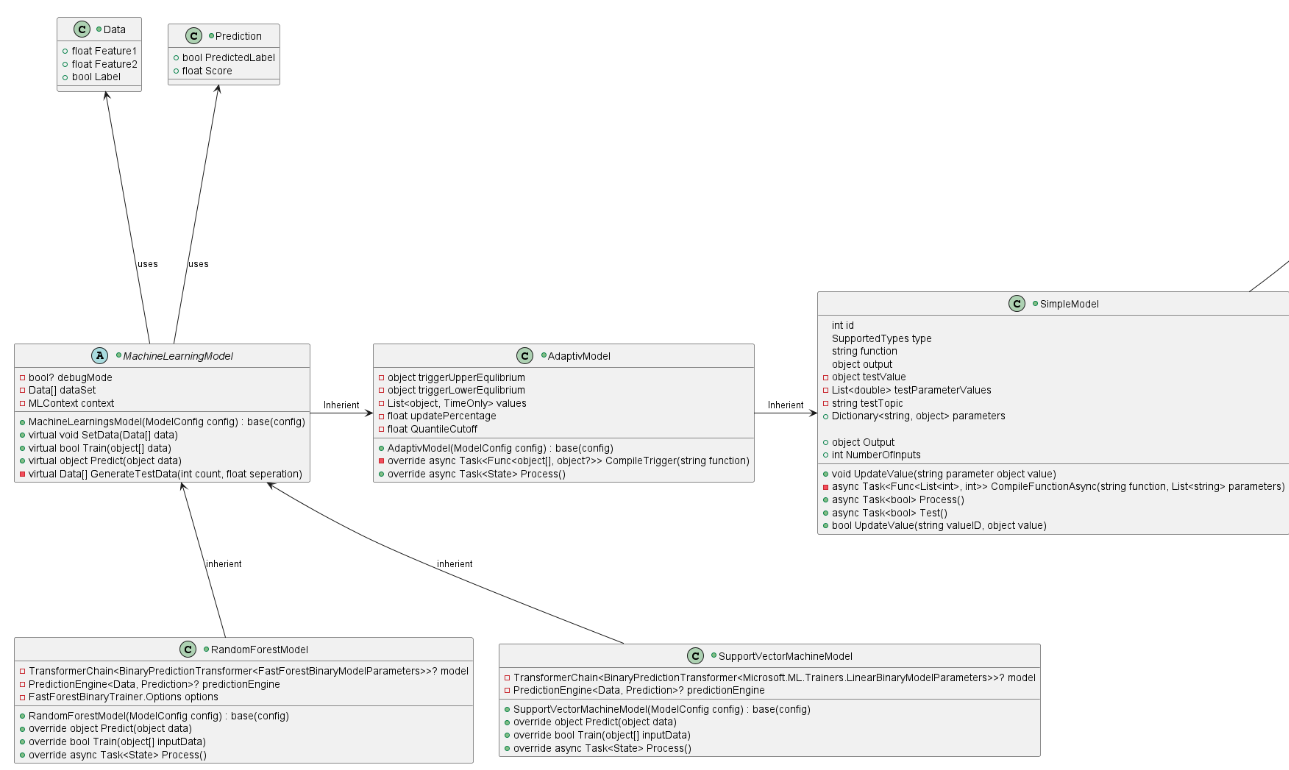
\includegraphics[width=.8\textwidth]{Images/models}
			\caption{Current Implemented models}
			\label{fig:implementedModels}
		\end{center}
	\end{figure}
	TODO: UPDATE IMAGE
	
	\subsubsection{Trigger}
	A trigger is implemented much the same way as a simple model, the difference is that the trigger is more limited in what it can return, this is because there is not the need for it and this limits the possibility arbitrary code execution.
	
	\subsubsection{JSON Reading}
		The JSONInterpreters job is to read a config file which a end user would be able to configure and then launch the \gls{reps}. The intention with this is to keep a users implementation of a \gls{reps} system simple. In a sense, the \gls{json} reading is a \gls{dsl} in which keeping complexity low is imperative for this project. Therefore the \gls{json} reading should contain few keywords to limit.
		{\scriptsize\begin{lstlisting}[language={[sharp]C},caption={Reading Sensor Configs},label=lst:readingSensorConfig]
private List<SensorConfig> ReadSensorConfigs(JObject config) {
	...
	foreach(JObject sensorNode in sensorNodes) {
		try {
			SensorConfig sensorConfig = new SensorConfig();
			sensorConfig.id = (int)sensorNode.GetValue("ID");
			sensorConfig.host = sensorNode.GetValue("Host").ToString();
			sensorConfig.name = sensorNode.GetValue("Name").ToString();
			sensorConfig.type = DetermineSupportedType(sensorNode);
			if(sensorConfig.type == SupportedTypes.STRING) {
				...
			}
			sensorConfig.topic = sensorNode.GetValue("Topic").ToString();
			sensorConfig.routingKey = sensorNode.GetValue("RoutingKey").ToString();
			sensorConfigs.Add(sensorConfig);
		}
		...
	}
	return sensorConfigs;
}
		\end{lstlisting}}
		Reading config files is implemented like Code Snippet \ref{lst:readingSensorConfig}, where the code can interpret specific values and then put the values into a struct which can be used to instantiate the models.
		
		{\scriptsize\begin{lstlisting}[language={[sharp]C}, caption={SensorConfig}, label=lst:SensorConfig]
public struct SensorConfig {
	public int id;
	public string name;
	public string host;
	public string routingKey;
	public string topic;
	public SupportedTypes type;
	public bool? isUsername;
}
		\end{lstlisting}}
	
		Implementing all of the configs in the \gls{json} reader, from which we can determine the amount of keywords needed implement the current solution. There is a total of 30 keywords, a list can be found in appendix \ref{sec:Keywords}.
		
		With the current implementation of the \gls{json} reader, a user can implement \gls{reps}. A simple model which takes 2 sensors and makes an addition to their values can be done like Code Snippet \ref{lst:simpleAddition}
{\scriptsize\begin{lstlisting}[language=json, caption={A simple model for addition}, label=lst:simpleAddition]
{
	"BrokerInfo": {
		"NotificationBroker": "localhost",
		"NotificationTopic": "notify",
		"ReportBroker": "localhost"
	},
	"SensorNodes": [{
		"ID": 0,
		"Name": "first",
		"SupportedType": "INT",
		"Host": "localhost",
		"RoutingKey": 0,
		"Topic": "first"
	},{
		"ID": 1,
		"Name": "second",
		"SupportedType": "INT",
		"Host": "localhost",
		"RoutingKey": 0,
		"Topic": "second"
	}],
	"EventNodes": [{
		"ID": 0,
		"Name": "Name",
		"SensorNodes": [ 0, 1 ],
		"EventNodes": [],
		"ReportTopic": "EventOutput",
		"SupportedType": "INT",
		"Host": "localhost",
		"RoutingKey" :  0,
		"Model": {
			"ID": 0,
			"Type": "Simple",
			"Name": "Name",
			"SupportedType": "INT",
			"Function": "a+b",
			"Parameters": [ "a", "b" ]
		}
	}
]
}\end{lstlisting}}
		A more realistic usage of \gls{reps} can be made as Code Snippet \ref{lst:BotCreation}. Which implements 1 sensor and 3 events to try and determine average time between bot creations, determine an event of a bot being created and when an attack of new bots being created.
		\newpage
{\scriptsize\begin{lstlisting}[language=json, caption={BotCreation Event},label=lst:BotCreation]
{"BrokerInfo": {
		"NotificationBroker": "localhost",
		"NotificationTopic": "notify",
		"ReportBroker": "localhost"
	},	
	"SensorNodes": [{
		"ID": 0,
		"Name": "AccountCreationSensor",
		"SupportedType": "STRING",
		"Host": "localhost",
		"RoutingKey": 0,
		"Topic": "AccountCreationActivity"
	}],
	"EventNodes": [{
		"ID": 0,
		"Name": "AccountCreationTimerEvent",
		"SensorNodes": [ 0 ],
		"EventNodes": [],
		"ReportTopic": "BotDetection",
		"SupportedType": "FLOAT",
		"Host": "localhost",
		"RoutingKey": 0,
		"Model": {
			"ID": 0,
			"Type": "timed",
			"DebugMode": false,
			"Name": "AccountCreationTimerModel",
			"SupportedType": "FLOAT",
			"TimedTrigger": 0.5,
			"Parameters": ["a"]
	}},	{
		"ID": 1,
		"Name": "BotDeterminerEvent",
		"SensorNodes": [ 2 ],
		"EventNodes": [],
		"ReportTopic": "BotDetection",
		"SupportedType": "INT",
		"Host": "localhost",
		"RoutingKey": 0,
		"Model": {
			"ID": 1,
			"Type": "svm",
			"DebugMode": false,
			"Name": "BotDeterminerModel",
			"SupportedType": "INT",
			"TrainingData": "C:/../TrainingsData.csv"
	}},{
		"ID": 2,
		"Name": "BotCreationAttackDeterminerEvent",
		"SensorNodes": [],
		"EventNodes": [ 0, 1 ],
		"ReportTopic": "BotCreationAttackDeterminer",
		"SupportedType": "INT",
		"Host": "localhost",
		"RoutingKey": 0,
		"Model": {
			"ID": 1,
			"Type": "simple",
			"DebugMode": false,
			"Name": "BotDeterminerModel",
			"SupportedType": "BOOLEAN",
			"Function": "return ((float)a > 0f && (float)b > 0.5)",
			"Parameters": [ "a", "b" ],
			"TriggerFunction": "if((bool)output) return 1; else return 0;"
	}}]}
\end{lstlisting}}
	\newpage
	\subsubsection{Nodes}
		Any kind of nodes implements an INode
		\begin{lstlisting}[language={[sharp]C},caption={INode}, label=lst:INode]
namespace REPS.Interfaces {
	public interface INode {
		object Output {
			get;
			set;
		}
		
		public Task Process();
		
	}
}
		\end{lstlisting}
		The 'Output' is where other nodes can access the value that the process gets/determines. The process returns a task which allows for it to run parallel with other task.
		\begin{lstlisting}[label={[sharp]C}, caption={Program.cs}, label=lst:foreachTask]
foreach(INode node in nodes) {
	if(node is EventNode) {
		tasks.Add(node.Process());
	}
}
		\end{lstlisting}
		
	\subsubsection{RabbitMQ}
		The implementation of the RabbitMQ implementation is split into 2 classes, Client, which handles any and all connections with a broker. Then there is the Connection class which handles direct communication with the broker.
		
		The Client has a simple implementation as RabbitMQ library already handles a lot of the background connections.
		\begin{lstlisting}[language={[sharp]C},caption={Client.cs},label=lst:Client]
namespace REPS.Connections {
	public class Client {
		private string hostname;
		private ConnectionFactory factory;
		private List<Connection> connections;
		private int id;
		public Client(string hostname) {
			this.hostname = hostname;
			this.factory = new ConnectionFactory { HostName = this.hostname };
			id = 0;
			connections = new List<Connection>();
		}
		
		public string Hostname { get { return hostname; } }
		
		public async Task<Connection> CreateConnectionAsync(string[] topics, string routingKey) {
			Connection connection = new Connection(id, topics, routingKey);
			id++;
			await connection.CreateConnectionAsync(this.factory);
			connections.Add(connection);
			return connection;
		}	
	}
}
		\end{lstlisting}
		Once a client has been instantiated, nodes can make connections. The methods used by the methods are Subscribe and SendMessage.
		
		\begin{lstlisting}[language={[sharp]C},caption={Connection.cs},label=lst:ConnectionSubscribe]
public async void Subscribe(string topic) {
	QueueDeclareOk queueDeclareResult = null;
	try {
		queueDeclareResult = await channel.QueueDeclareAsync();
	}
	catch(NullReferenceException ex) {
		...
		return;
	}
	string queueName = queueDeclareResult.QueueName;
	await channel.QueueBindAsync(queue: queueName, exchange: topic, routingKey: routingKey);
	AsyncEventingBasicConsumer consumer = new AsyncEventingBasicConsumer(channel);
	consumer.ReceivedAsync += (model, ea) => {
		byte[] body = ea.Body.ToArray();
		string message = Encoding.UTF8.GetString(body);
		this.returnMessage = message;
		return Task.CompletedTask;
	};
	await channel.BasicConsumeAsync(queue: queueName, autoAck: true, consumer: consumer);
}
		\end{lstlisting}
		With this implementation sensor nodes can receive data from the broker.
		\begin{lstlisting}[language={[sharp]C},caption={SensorNode.cs},label=lst:initSensor]
private async Task<bool> initAsync() {
	connection = connectionTask.Result;
	connectionTask.Dispose();
	connection.Subscribe(topic);
	return true;
}
		\end{lstlisting}
		
		And it is possible for event nodes to send their determination to the broker.
		\begin{lstlisting}[language={[sharp]C},caption={EventNode.cs},label=lst:EventNodeSendMessage]
    ...   
    this.state = await model.Process();
}

if(state == State.Stable) {
await connection.SendMessageAsync($"EventNode {id}, {name}, reports stable condition : Statelevel: {State.Stable}");
}
else {
await connection.SendMessageAsync($"EventNode {id}, {name}, reports unstable condition : Statelevel: {state}");
}
		\end{lstlisting}
	\subsubsection{Miscellaneous}
		In this section I'll go into things that is note worthy but not enough for their own section.
		
		\textbf{Threading}\\ \noindent
			Each node can run within its own threads, avoiding the problem of them having to wait for one another, the problem with this is the faster nodes may reuse data from other nodes which hasn't finished. This is accepted thinking that each data point is not necessary to determine events.
		
		\textbf{Name Extraction}\\ \noindent
			I found it useful to determine any characteristics about usernames in the \gls{reps} rather than in a separate service. It helped in the specific use case in Code Snippet \ref{lst:BotCreation}, this lead to a more of a extraction module which could follow a code injection pattern if further developed, allowing for a broader and more defined use case for the \gls{ml} models in \gls{reps}.
			
		\textbf{Supported Types}\\ \noindent
			A supported type is just a type which the \gls{reps} supports, the idea is that you could have complicated types rather than just simple. This now seems to be unneassery as the need for support for complex types is doesn't seem to be a need.
	
	\subsection{Simulator}
		A simulator was made to simulate website trafic so the implementation of \gls{reps} could be confirmed and ensure that it worked as intended. This is developed because while unit testing ensures that the individual components of \gls{reps} works as intended, putting the whole system into a likely scenario often reveals problems which is not covered by the unit test. Making a simulator to as a like to a real system, I created some code which would make request to a website, this website then publishes information about this 'attack' to the RabbitMQ broker.
		\begin{figure}[!h]
			\begin{center}
				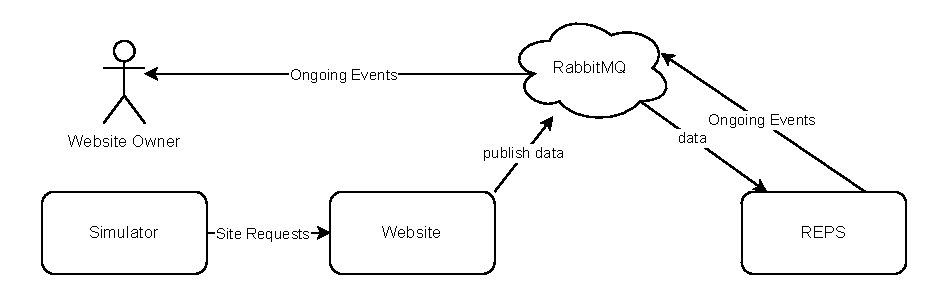
\includegraphics[width=.8\textwidth]{Images/Simulator}
			\end{center}
		\end{figure}
		The simulator will have several different type of events which can occur such as login attempts and creation of new accounts.
		\begin{lstlisting}[language={[sharp]C},caption={Simulator.Event.cs},label=lst:Simulator]
class WebSiteLoginEvent : WebSiteActionEvent {
	public WebSiteLoginEvent(string site, int seed, int minimumRequests, int maxmimumRequests) : base(site, seed, minimumRequests, maxmimumRequests, null) {
		this.message = new JObject();
	}
	
	public override async void Start() {
		for(int j = 0; j < numberOfAttacks; j++) {
			string name = ""; string password = "";
			int length = random.Next(20) + 2;
			for(int i = 0; i < length; i++) {
				name += random.Next(2) == 1 ? letters[random.Next(letters.Length)] : letters[random.Next(letters.Length)].ToString().ToUpper();
			}
			for(int i = 0; i < length; i++) {
				password += random.Next(2) == 1 ? letters[random.Next(letters.Length)] : letters[random.Next(letters.Length)].ToString().ToUpper();
			}
			this.message["username"] = name;
			this.message["password"] = password;
			await client.PostAsync(site + "/login", new StringContent(message.ToString(), Encoding.UTF8, "application/json"));
		}
	}
}
		\end{lstlisting}
		The simulator also supports saving the data into a csv file, which can be used to train the \gls{ml} models.
	
	\subsection{\gls{gui}}
		The \gls{gui} is developed to help during testing and experimentation. It is just as much a development tool as it is part of the final product for the user. The \gls{gui} is developed in C\#'s blazor as it supports linux platform which other C\# platforms does not, and it is the frameworks that I have most experience with. It being same language as the REPS allows for the system to use the config files implemented in the REPS mentioned in section \ref{Reps:Imp}. As it is a development tool I do not intend to make updates to it when I update the REPS, so having it dynamically change depending on config files will ease development and testing. The \gls{gui} will decrease the amount of misconfigurations and increase the speed of which new configurations can be made. The \gls{gui} will create a json file which can be used to launch a \gls{reps}.
		
		Blazor was also chosen for being component based, I can easily add new pages or reuse components if the need arises.
		Other frameworks which could be used to develop a \gls{gui} is WinUI, WindowsForms \& Maui, the problem with all of these is I lack experience with them or they do not support Linux.
		
		The \gls{gui} never finished as it is not considered a must for \gls{reps}. Development on it started but stopped once I realised it would not give a high enough return on the value. Still some ideas from the minimal development was revealed.
		\begin{lstlisting}[language={[sharp]C},caption={JSON.razor},label=lst:GUITypeDetermination]
public List<(string, string, Guid, int)> GetTypes<T>() {
	List<(string, string, Guid, int)> types = new(); // I did not use dictionary to avoid the risk of macthing keys
	
	if (typeof(T) == typeof(SensorConfig)) {
		foreach (FieldInfo? field in fieldsTypes[0].GetFields(BindingFlags.Public | BindingFlags.Instance)) {
			Guid guid = Guid.NewGuid();
			AddGuidToKey(configNumber, guid);
			types.Add((field.Name, field.FieldType.Name, guid, configNumber));
		}
	}
	else if (typeof(T) == typeof(EventConfig)) {
		foreach (FieldInfo? field in fieldsTypes[1].GetFields(BindingFlags.Public | BindingFlags.Instance)) {
			types.Add((field.Name, field.FieldType.Name, Guid.NewGuid(), configNumber));
		}
	}
	else if (typeof(T) == typeof(ModelConfig)) {
		foreach (FieldInfo? field in fieldsTypes[2].GetFields(BindingFlags.Public | BindingFlags.Instance)) {
			types.Add((field.Name, field.FieldType.Name, Guid.NewGuid(), configNumber));
		}
	}
	return types;
}
		\end{lstlisting}
		This method as access to the same struct config types in \gls{reps} such as Sensor Config [Code Snippet \ref{lst:SensorConfig}]. From this you can automatically form a table where a user could add in the relevant information.
		
	\subsection{Testing}
		Testing methodologies and techniques in software engineering come in many forms, with popular examples including test-driven development, unit testing, and UI testing. These approaches help ensure that the final product meets its requirements.
		For this project, unit testing plays an important role but is not sufficient to cover the system as a whole, which is particularly important for the \gls{reps}. Since \gls{reps} is a supportive system designed to flag issues within the environment it operates in, A separate system which can test the \gls{reps} is developed.\newline \newline
		
	\subsection{Research Question 0 : How should a \gls{reps} be constructed}
		A \gls{reps} should be constructed based on this projects experience along side other patterns and software engineering values/tactics. Separation of concerns is a value which comes with a \gls{reps} by its design. Nodes only retrieves their data and do not publish to other nodes, this allows for easier adding and removing of new nodes.
		
		The using a human readable configuration file allows a user to make quick changes, during and in between runtimes. The patterns design allows for simple setup and interaction with the system while keeping the time to learn the system lower than many other similar solutions.
		
		To conclude the best way to implement \gls{reps}, it should be implemented with every node being independent, this allows for varied implementations, this project is implemented for a monolith structure, but there no reason for not being implemented like micro service. The nodes being independent allows for the nodes to do their calculations at once without needing to wait for other nodes to finish. There should to be a clear separation between the sensor nodes and event nodes as their concern is different and many event nodes can use the same sensor for their determination. The event nodes should only have one output, this ensures that the event node keeps to its focus.